\chapter{Architecture}
A high level abstraction of the general architecture of the system is available in \autoref{fig:Architecture}.
The system is composed from 2 building block:
\begin{itemize}
    \item \textbf{LoRaWan network simulator} $\rightarrow$ simulate the LoRaWan network where are presents sensors, user device and network facilities required from a LoRaWan network. It simulates the bi-directional communication between all the kinds of network entities.
    \item \textbf{AC application} $\rightarrow$ application that receive data from sensor and user devices, identifies areas with good air quality and defines the required routes
\end{itemize}

\begin{figure}[h]
    \centering
    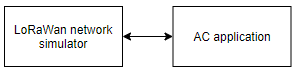
\includegraphics[scale=1.2]{architectureHL.png}
    \caption{System architecture}
    \label{fig:Architecture}
\end{figure}

This two building block exchange 3 kind of message:
\begin{enumerate}
    \item \textbf{Sensor message}: message from sensors to application with the new sensed value
    \item \textbf{Request route message}: message from user device to application to require a route for a specified destination
    \item \textbf{Route message}: message from application to user device with the route to follow to reach the destination
\end{enumerate}

